% =====================================================================
%  MR2006B Industrial Automation -- Module 4: Control
%  Assessment 1: Modeling of Dynamic Systems using Least Squares
%  Method and ARX structures -- IEEE conference template (IEEEtran)
%
%  Numbers, tables and result figures come from results.tex and the
%  fig_*.pdf files. Both are written by matlab/sysid_A1.m. Run it after
%  the experiments, then compile this file. Red "??" = not computed yet.
% =====================================================================
\documentclass[conference]{IEEEtran}
\IEEEoverridecommandlockouts
\usepackage{cite}
\usepackage{amsmath,amssymb,amsfonts}
\usepackage{graphicx}
\usepackage{textcomp}
\usepackage{xcolor}
\usepackage{booktabs}
\usepackage{tikz}
\usetikzlibrary{positioning,arrows.meta,calc,fit,backgrounds}
\usepackage[hidelinks]{hyperref}
\def\BibTeX{{\rm B\kern-.05em{\sc i\kern-.025em b}\kern-.08em
    T\kern-.1667em\lower.7ex\hbox{E}\kern-.125em X}}

% ---------- results (overwritten by results.tex) ----------
\newcommand{\NA}{\textcolor{red}{??}}
\newcommand{\NArow}[1]{\multicolumn{#1}{c}{\textcolor{red}{run \texttt{sysid\_A1.m}}} \\}
\newcommand{\DataReady}{0}
\newcommand{\LonOrder}{ARX(\NA)}  \newcommand{\LatOrder}{ARX(\NA)}
\newcommand{\LonNa}{\NA}  \newcommand{\LonNb}{\NA}  \newcommand{\LonNk}{\NA}
\newcommand{\LatNa}{\NA}  \newcommand{\LatNb}{\NA}  \newcommand{\LatNk}{\NA}
\newcommand{\LonNtrain}{\NA} \newcommand{\LatNtrain}{\NA}
\newcommand{\LonNval}{\NA}   \newcommand{\LatNval}{\NA}
\newcommand{\LonSigma}{\NA}  \newcommand{\LatSigma}{\NA}
\newcommand{\LonRpred}{\NA}  \newcommand{\LatRpred}{\NA}
\newcommand{\LonRsim}{\NA}   \newcommand{\LatRsim}{\NA}
\newcommand{\LonRval}{\NA}   \newcommand{\LatRval}{\NA}
\newcommand{\LonRvalmin}{\NA}\newcommand{\LatRvalmin}{\NA}
\newcommand{\LonK}{\NA}      \newcommand{\LatK}{\NA}
\newcommand{\LonTau}{\NA}    \newcommand{\LatTau}{\NA}
\newcommand{\LonPoles}{\NA}  \newcommand{\LatPoles}{\NA}
\newcommand{\LonWhite}{\NA}  \newcommand{\LatWhite}{\NA}
\newcommand{\LonIndep}{\NA}  \newcommand{\LatIndep}{\NA}
\newcommand{\LonModel}{\NA}  \newcommand{\LatModel}{\NA}
\newcommand{\LonCov}{\NA}    \newcommand{\LatCov}{\NA}
\newcommand{\LonParamRows}{\NArow{3}} \newcommand{\LatParamRows}{\NArow{3}}
\newcommand{\LonValRows}{\NArow{3}}   \newcommand{\LatValRows}{\NArow{3}}
\newcommand{\LonOrderRows}{\NArow{4}} \newcommand{\LatOrderRows}{\NArow{4}}
\InputIfFileExists{results.tex}{}{}

% figure from file, or a framed placeholder if the file is missing
\newcommand{\figfile}[3][\columnwidth]{%
  \IfFileExists{#2}{\includegraphics[width=#1]{#2}}%
  {\fbox{\parbox[c][#3][c]{\dimexpr#1-2\fboxsep-2\fboxrule}{\centering\small
   \textcolor{red}{\texttt{\detokenize{#2}}}\\ \footnotesize missing}}}}

% to do for the team (red, remove before submitting)
\newcommand{\todo}[1]{\textcolor{red}{[TODO: #1]}}

\begin{document}

\title{Least-Squares ARX Identification of the Longitudinal and Lateral
Dynamics of a Differential-Drive Autonomous Vehicle Prototype\thanks{Assessment 1,
Industrial Automation (MR2006B.602), Module 4: Control, Prof. Juan Carlos Tud\'on,
Tecnol\'ogico de Monterrey, November 2026.}}

\author{
\IEEEauthorblockN{Isaac Sebastian Hovmand}
\IEEEauthorblockA{\textit{A01832781} \\
Tecnol\'ogico de Monterrey\\
Monterrey, Mexico}
\and
\IEEEauthorblockN{Thomas Michael Resch}
\IEEEauthorblockA{\textit{A01832776} \\
Tecnol\'ogico de Monterrey\\
Monterrey, Mexico}
\and
\IEEEauthorblockN{Jan Mosler}
\IEEEauthorblockA{\textit{A01833812} \\
Tecnol\'ogico de Monterrey\\
Monterrey, Mexico}
\and
\IEEEauthorblockN{Daniel Appel}
\IEEEauthorblockA{\textit{A01833285} \\
Tecnol\'ogico de Monterrey\\
Monterrey, Mexico}
}

\maketitle

\begin{abstract}
This paper identifies the longitudinal and lateral dynamics of the
EuroMotion vehicle, a battery-powered differential-drive prototype for
autonomous navigation built around an STM32F446RE microcontroller.
The longitudinal model maps the mean PWM duty of both wheels to the
vehicle speed. The lateral model maps the differential duty to the yaw
rate. Both are discrete-time ARX models estimated by ordinary least
squares at a sampling time of 20\,ms. A dedicated test firmware applies
six open-loop excitations: multi-level step, PRBS and chirp for the
longitudinal dynamics, and PRBS, double lane change (DLC) and single lane
change (SLC) for the lateral dynamics. The models are trained on the PRBS
runs only and cross-validated on all other runs. The selected models are
\LonOrder\ (longitudinal) and \LatOrder\ (lateral). In free-run simulation
they reach a mean validation $R^2$ of \LonRval\ and \LatRval, respectively.
\end{abstract}

\begin{IEEEkeywords}
system identification, least squares, ARX model, vehicle dynamics,
cross-validation, differential drive, STM32
\end{IEEEkeywords}

% =====================================================================
\section{Introduction}
% =====================================================================
A controller can only be as good as the model it is designed for.
Vehicle dynamics models predict how a vehicle reacts to its inputs. This
allows controllers to be designed and tested in simulation before they
run on the real vehicle \cite{rajamani,gillespie}.

The EuroMotion vehicle is the team's prototype for the MR2006B challenge.
It must drive a closed circuit autonomously, stop at waypoints and avoid
obstacles. This needs two control loops: one for the speed and one for the
heading. Each loop needs a model.

Physical models need parameters that are hard to measure on a small
vehicle: mass, inertia, motor constants, rolling and scrubbing friction.
System identification avoids this. It fits a model structure directly to
measured input--output data \cite{ljung}. Here we use the least-squares
(LS) method with ARX model structures. LS has a closed-form solution and
gives the covariance of the estimates.

The contributions are:
(i) a description of the hardware and the integrated control system,
including the choice of the sampling time;
(ii) a test firmware with six reproducible excitation signals;
(iii) LS identification of the longitudinal and lateral dynamics with
order selection; and
(iv) cross-validation on several new data sets for both dynamics.

% =====================================================================
\section{System Description}
% =====================================================================
\subsection{Vehicle and Components}
The vehicle has four wheels and differential (skid) steering. The left and
right wheels are driven by one DC gear motor each. Steering is achieved by
a speed difference between both sides. Table~\ref{tab:comp} lists the
components and their role in the control system. Fig.~\ref{fig:car} shows
the vehicle and Fig.~\ref{fig:schem} the wiring.

\begin{table}[t]
\caption{Components and their role in the control system}
\label{tab:comp}
\centering
\footnotesize
\begin{tabular}{@{}p{2.3cm}p{1.1cm}p{4.0cm}@{}}
\toprule
\textbf{Component} & \textbf{Role} & \textbf{Function} \\
\midrule
NUCLEO-F446RE (STM32F446RE, 180\,MHz) & Controller & Runs the 50\,Hz loop (TIM6 interrupt), reads encoders (TIM3/TIM8), generates PWM (TIM1, 20\,kHz). \\
2$\times$ JGB37-3530 DC gear motor, 12\,V, 56:1 & Actuator & Drive the left and right side. \\
2$\times$ BTS7960 H-bridge & Actuator & Power stage. Converts the PWM duty $u\in[-100,100]\,\%$ into motor voltage. \\
2$\times$ Hall encoder (16 PPR, $\times$4) & Sensor & 3584 counts per wheel revolution, $k_x = 0.0636$\,mm/count. Measure wheel speed and yaw rate. \\
HC-SR04 ultrasonic & Sensor & Obstacle distance (not used in the identification). \\
HC-12 radio, 433\,MHz & Comms & Telemetry and remote commands, 9600\,baud. \\
USB / ST-LINK VCP & Comms & Data logging, 115200\,baud. \\
12\,V battery + XY-3606 buck & Power & Motor supply and 5\,V logic supply. \\
\bottomrule
\end{tabular}
\end{table}

\begin{figure}[t]
\centering
\figfile{fig_car.jpg}{4.2cm}
\caption{EuroMotion vehicle: NUCLEO board, BTS7960 drivers, gear motors
with encoders, HC-12 radio and battery.}
\label{fig:car}
\end{figure}

\begin{figure*}[t]
\centering
\figfile[0.82\textwidth]{fig_schematic.pdf}{8cm}
\caption{Wiring schematic of the vehicle (battery, buck converter,
NUCLEO-F446RE, two BTS7960 drivers, encoders, HC-12, OLED and HC-SR04).}
\label{fig:schem}
\end{figure*}

\subsection{Integrated Control System}
Fig.~\ref{fig:block} shows the control system to be designed with the
identified models. The user or the path planner sets a speed reference
$v_{\mathrm{ref}}$ and a yaw-rate reference $r_{\mathrm{ref}}$. A speed
controller computes the mean duty $\bar u$. A yaw-rate controller computes
the differential duty $\Delta u$. A mixer converts both into wheel duties:
\begin{equation}
u_L = \bar u - \Delta u, \qquad u_R = \bar u + \Delta u .
\label{eq:mix}
\end{equation}
The encoders measure the wheel speeds $v_L$ and $v_R$. The kinematics of a
differential drive with track width $b = 0.223$\,m give
\begin{equation}
v = \frac{v_R + v_L}{2}, \qquad r = \frac{v_R - v_L}{b} .
\label{eq:kin}
\end{equation}
The mixer \eqref{eq:mix} and the kinematics \eqref{eq:kin} decouple the
plant into two single-input single-output systems: $G_v(z)$ from $\bar u$
to $v$ (longitudinal) and $G_r(z)$ from $\Delta u$ to $r$ (lateral).
These two transfer functions are identified in this work.

\begin{figure*}[t]
\centering
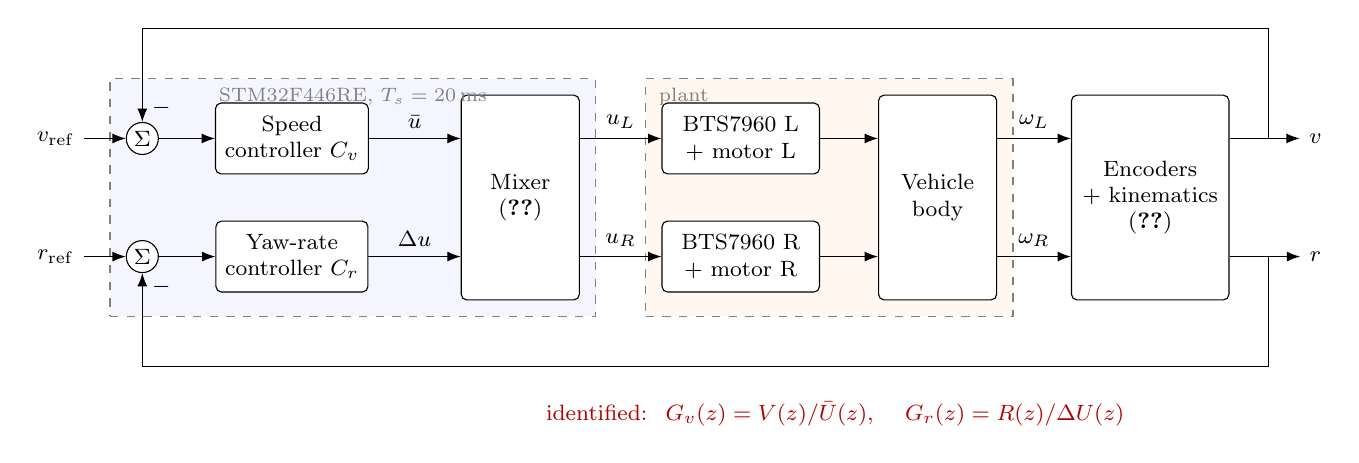
\begin{tikzpicture}[>=Latex, font=\footnotesize,
  blk/.style={draw, rounded corners=2pt, minimum height=0.9cm, minimum width=1.9cm, align=center, fill=white},
  tall/.style={blk, minimum height=2.6cm, minimum width=1.5cm},
  sum/.style={draw, circle, inner sep=1.2pt, fill=white}]
  \node (vr) at (0,0.75) {$v_{\mathrm{ref}}$};
  \node (rr) at (0,-0.75) {$r_{\mathrm{ref}}$};
  \node[sum] (s1) at (1.1,0.75) {$\Sigma$};
  \node[sum] (s2) at (1.1,-0.75) {$\Sigma$};
  \node[blk] (cv) at (3.0,0.75) {Speed\\controller $C_v$};
  \node[blk] (cr) at (3.0,-0.75) {Yaw-rate\\controller $C_r$};
  \node[tall] (mix) at (5.9,0) {Mixer\\ \eqref{eq:mix}};
  \node[blk, minimum width=2.0cm] (dl) at (8.7,0.75) {BTS7960 L\\+ motor L};
  \node[blk, minimum width=2.0cm] (dr) at (8.7,-0.75) {BTS7960 R\\+ motor R};
  \node[tall] (veh) at (11.2,0) {Vehicle\\body};
  \node[tall, minimum width=2.0cm] (enc) at (13.9,0) {Encoders\\+ kinematics\\ \eqref{eq:kin}};
  \node (vo) at (16.0,0.75) {$v$};
  \node (ro) at (16.0,-0.75) {$r$};
  \draw[->] (vr) -- (s1); \draw[->] (rr) -- (s2);
  \draw[->] (s1) -- (cv); \draw[->] (s2) -- (cr);
  \draw[->] (cv) -- node[above]{$\bar u$} (cv -| mix.west);
  \draw[->] (cr) -- node[above]{$\Delta u$} (cr -| mix.west);
  \draw[->] (dl -| mix.east) -- node[above]{$u_L$} (dl);
  \draw[->] (dr -| mix.east) -- node[above]{$u_R$} (dr);
  \draw[->] (dl) -- (dl -| veh.west);
  \draw[->] (dr) -- (dr -| veh.west);
  \draw[->] (veh.east |- dl) -- node[above]{$\omega_L$} (enc.west |- dl);
  \draw[->] (veh.east |- dr) -- node[above]{$\omega_R$} (enc.west |- dr);
  \draw[->] (enc.east |- vo) -- (vo);
  \draw[->] (enc.east |- ro) -- (ro);
  \draw[->] (15.4,0.75) -- (15.4,2.15) -- (1.1,2.15) -- node[pos=0.85, right]{$-$} (s1);
  \draw[->] (15.4,-0.75) -- (15.4,-2.15) -- (1.1,-2.15) -- node[pos=0.85, right]{$-$} (s2);
  \begin{scope}[on background layer]
    \node[draw, dashed, gray, fill=blue!4, inner sep=0.2cm, fit=(s1)(s2)(cv)(cr)(mix)] (mcu) {};
    \node[draw, dashed, gray, fill=orange!6, inner sep=0.2cm, fit=(dl)(dr)(veh)] (pl) {};
  \end{scope}
  \node[gray, anchor=north, font=\scriptsize] at (mcu.north) {STM32F446RE, $T_s = 20$\,ms};
  \node[gray, anchor=north west, font=\scriptsize] at ($(pl.north west)+(0.05,0)$) {plant};
  \node[text=red!70!black] at (9.9,-2.75)
     {identified: \ $G_v(z)=V(z)/\bar U(z)$, \quad $G_r(z)=R(z)/\Delta U(z)$};
\end{tikzpicture}
\caption{Block diagram of the integrated control system. The mixer and the
kinematics split the vehicle into a longitudinal plant $G_v$ and a lateral
plant $G_r$. The references come from the user (HC-12 radio) or the path
planner. The controllers $C_v$ and $C_r$ will be designed with the models
identified in this paper.}
\label{fig:block}
\end{figure*}

\subsection{Sampling Time}\label{sec:ts}
The control loop and the data logger run at $T_s = 20$\,ms. TIM6 is clocked
at 90\,MHz with prescaler 8999 and auto-reload 199 \cite{rm0390}:
$f = 90\,\mathrm{MHz}/(9000\cdot 200) = 50$\,Hz. Four criteria justify this
value.

\emph{1) Plant dynamics.} An earlier open-loop test with the wheels lifted
gave a motor time constant of $\tau \approx 50$\,ms. On the floor the mass
of the vehicle makes the response slower. A common rule asks for 4 to 10
samples per rise time $t_r \approx 2.2\tau$ \cite{astrom}. With
$\tau = 50$\,ms this gives $T_s = 11$ to 28\,ms. 20\,ms lies in this range
even for the fastest (unloaded) case.

\emph{2) Closed-loop bandwidth.} The sampling frequency should be 10 to 30
times the closed-loop bandwidth \cite{astrom}. With
$\omega_s = 2\pi/T_s = 314$\,rad/s, loops up to about 10 to 30\,rad/s are
possible. This is faster than needed for a vehicle at walking speed.

\emph{3) Speed resolution.} The speed is the count difference per period.
Its resolution is $k_x/T_s = 3.2$\,mm/s at 20\,ms. At 5\,ms it would be
12.7\,mm/s, which is 4\,\% of a typical speed of 300\,mm/s. A shorter
$T_s$ therefore adds quantization noise. A longer $T_s$ adds delay.

\emph{4) Data transfer.} One log line has about 22 characters. At
115200\,baud it takes 1.9\,ms, at 9600\,baud (HC-12) 23\,ms. Live
streaming over the radio would not fit into 20\,ms. The test firmware
therefore stores the data in RAM and sends it after the test.

% =====================================================================
\section{Modeling and Identification Method}
% =====================================================================
\subsection{Model Structures}
\emph{Longitudinal.} Newton's law for the vehicle mass $m$ with both
traction forces and the resistance forces is
$m\dot v = F_L + F_R - F_{\mathrm{res}}$ \cite{rajamani}. The motor
electrical time constant is much smaller than the mechanical one.
Linearized around an operating point this gives a first-order system
\begin{equation}
G_v(s) = \frac{V(s)}{\bar U(s)} = \frac{K_v}{\tau_v s + 1}.
\label{eq:lon}
\end{equation}
Its zero-order-hold discretization is an ARX(1,1,1) model with
$a_1 = -e^{-T_s/\tau_v}$ and $b_1 = K_v(1+a_1)$.

\emph{Lateral.} For a differential drive the yaw moment comes from the
force difference: $I_z \dot r = \tfrac{b}{2}(F_R - F_L) - M_{\mathrm{scrub}}$.
Together with the motor dynamics this gives a second-order system from
$\Delta u$ to $r$. It plays the same role as the bicycle model for
Ackermann vehicles \cite{rajamani}. Since tire scrubbing of a skid-steer
vehicle is hard to model, the order is chosen from the data.

\subsection{ARX Model and Least Squares}
The ARX($n_a$,$n_b$,$n_k$) model is \cite{ljung}
\begin{equation}
y(k) + \sum_{i=1}^{n_a} a_i\, y(k-i) = \sum_{j=1}^{n_b} b_j\, u(k-n_k-j+1) + e(k).
\end{equation}
In regression form $y(k) = \varphi^{T}(k)\,\theta + e(k)$ with
\begin{align}
\varphi(k) &= [-y(k-1)\; \dots\; -y(k-n_a) \nonumber\\
           &\qquad u(k-n_k)\; \dots\; u(k-n_k-n_b+1)]^{T}, \nonumber\\
\theta &= [a_1\; \dots\; a_{n_a}\;\; b_1\; \dots\; b_{n_b}]^{T}.
\end{align}
Stacking $N$ samples gives $Y = \Phi\theta + E$. The LS estimate minimizes
$\|Y - \Phi\theta\|^2$:
\begin{equation}
\hat\theta = (\Phi^{T}\Phi)^{-1}\Phi^{T} Y .
\label{eq:ls}
\end{equation}
With the residual variance
$\hat\sigma^2 = \|Y - \Phi\hat\theta\|^2/(N - n_a - n_b)$ the covariance of
the estimate is \cite{soderstrom}
\begin{equation}
P = \hat\sigma^2\,(\Phi^{T}\Phi)^{-1}.
\label{eq:cov}
\end{equation}
The square roots of the diagonal of $P$ are the standard deviations of the
parameters.

\subsection{Order Selection and Validation}
All combinations $n_a \in \{1,2,3\}$, $n_b \in \{1,2,3\}$ and
$n_k \in \{1,2\}$ are estimated on the training data. Each model is
simulated on the validation data. The model with the fewest parameters
within 0.005 of the best mean validation $R^2$ is selected. This avoids
overfitting.

The models are judged by free-run simulation, not one-step prediction.
The simulated output $\hat y$ uses only the measured input. This is the
harder test, because errors accumulate. The fit index is
\begin{equation}
R^2 = 1 - \frac{\sum_k (y(k) - \hat y(k))^2}{\sum_k (y(k) - \bar y)^2}.
\label{eq:r2}
\end{equation}
In addition, the residuals of the training data are tested for whiteness
(autocorrelation $R_{ee}$) and for independence from the input
(cross-correlation $R_{ue}$), with 99\,\% bounds $\pm 2.58/\sqrt N$
\cite{ljung}.

% =====================================================================
\section{Experiments}
% =====================================================================
\subsection{Test Firmware and Procedure}
A test module was added to the vehicle firmware. It runs inside the 50\,Hz
interrupt and overrides the controllers, so all tests are open loop. A
serial command \texttt{X1}--\texttt{X6} starts one test. Every test begins
with a 1.5\,s warm-up at a constant duty. The excitation follows. Then the
motors stop. The firmware stores both duties and both raw encoder
increments for every sample (8 bytes per sample) and sends the log as CSV
after the test. A MATLAB script on the PC starts the test and saves the
file.

The raw encoder increments are used, not the filtered speed of the
firmware. This keeps the IIR filter out of the identified dynamics. All
tests ran on the same floor with a fully charged battery.
\todo{state floor type, battery voltage and date of the tests.}

\subsection{Excitation Signals}
Fig.~\ref{fig:tests} shows the six inputs.

\emph{Longitudinal} (same duty on both wheels, $40 \pm 10\,\%$):
a multi-level step (5 levels, 2\,s each);
a PRBS of 127 bits with a bit time of 60\,ms;
and a linear chirp from 0.2 to 3\,Hz over 10\,s.

\emph{Lateral} (base duty 35\,\%, differential duty $\Delta u = \pm 8\,\%$):
a PRBS of 127 bits with a bit time of 80\,ms;
a double lane change (DLC) based on the ISO\,3888-1 maneuver \cite{iso3888};
and a single lane change (SLC).
For the skid-steer vehicle, the steering wheel angle of the standard
maneuvers is replaced by $\Delta u$.

The PRBS is generated by a 7-bit shift register
($x^7 + x^6 + 1$). Its spectrum is nearly flat up to about
$0.44/T_b$, i.e. 7.3\,Hz (60\,ms) and 5.5\,Hz (80\,ms). This covers the
expected plant bandwidth of 1 to 3\,Hz. A PRBS of period 127 is
persistently exciting of high order \cite{ljung}, so all ARX orders tested
here are identifiable from it.

\begin{figure*}[t]
\centering
\figfile[0.95\textwidth]{fig_tests.pdf}{5cm}
\caption{Excitation signals of the six tests. The dashed line marks the end
of the 1.5\,s warm-up. Longitudinal tests: duty of both wheels. Lateral
tests: differential duty added to a base duty of 35\,\%.}
\label{fig:tests}
\end{figure*}

\subsection{Preprocessing and Cross-Validation}
Speed and yaw rate are computed with \eqref{eq:kin} from the encoder
increments. The operating point is the mean of input and output during
the last 0.5\,s of the warm-up. It is subtracted, so the models describe
deviations around $\bar u = 40\,\%$ (longitudinal) and
$\Delta u = 0$ (lateral). This also removes the dead zone of the drivers
and the small offset in yaw rate caused by the two motors not being
identical.

Every test was run twice. Table~\ref{tab:cv} shows the use of the data.
The models see only the first PRBS run. Five new data sets per dynamics
remain for cross-validation: two other signal types, each run twice, and a
second PRBS run.

\begin{table}[t]
\caption{Use of the data sets}
\label{tab:cv}
\centering
\footnotesize
\begin{tabular}{@{}lll@{}}
\toprule
\textbf{Dynamics} & \textbf{Training} & \textbf{Cross-validation} \\
\midrule
Longitudinal & PRBS run 1 & Step 1, 2; Chirp 1, 2; PRBS 2 \\
Lateral      & PRBS run 1 & DLC 1, 2; SLC 1, 2; PRBS 2 \\
\bottomrule
\end{tabular}
\end{table}

% =====================================================================
\section{Results}
% =====================================================================
\subsection{Order Selection}
Table~\ref{tab:order} lists the best structures. For the longitudinal
dynamics \LonOrder\ was selected, for the lateral dynamics \LatOrder.
\todo{one sentence: does the selected order match the physical expectation
(1st order longitudinal, 2nd order lateral)? If a higher order is only
marginally better, say so.}

\begin{table}[t]
\caption{Order selection ($R^2$, free-run simulation). $\star$ = selected}
\label{tab:order}
\centering
\footnotesize
\begin{tabular}{@{}lccc@{}}
\toprule
($n_a$,$n_b$,$n_k$) & \# par. & $R^2$ train & $R^2$ val. (mean) \\
\midrule
\multicolumn{4}{@{}l}{\emph{Longitudinal}} \\
\LonOrderRows
\midrule
\multicolumn{4}{@{}l}{\emph{Lateral}} \\
\LatOrderRows
\bottomrule
\end{tabular}
\end{table}

\subsection{Longitudinal Model}
The LS estimate \eqref{eq:ls} on $N = \LonNtrain$ samples gives
\begin{equation}
G_v(z) = \LonModel \quad \left[\frac{\mathrm{m/s}}{\%}\right]
\end{equation}
with pole(s) at $z = \LonPoles$. The static gain is
$K_v = \LonK$\,(m/s)/\% and the dominant time constant is
$\tau_v = \LonTau$\,ms. Table~\ref{tab:param} gives the parameters with their
standard deviations. The covariance matrix \eqref{eq:cov} is
\begin{equation}
P_v = \LonCov .
\end{equation}

\begin{table}[t]
\caption{Estimated parameters and standard deviations $\sigma_\theta = \sqrt{P_{ii}}$}
\label{tab:param}
\centering
\footnotesize
\begin{tabular}{@{}lrr@{}}
\toprule
Parameter & $\hat\theta$ & $\sigma_\theta$ \\
\midrule
\multicolumn{3}{@{}l}{\emph{Longitudinal} $G_v$, $\hat\sigma_e = \LonSigma$\,m/s} \\
\LonParamRows
\midrule
\multicolumn{3}{@{}l}{\emph{Lateral} $G_r$, $\hat\sigma_e = \LatSigma$\,rad/s} \\
\LatParamRows
\bottomrule
\end{tabular}
\end{table}

Fig.~\ref{fig:lontrain} compares the simulated and the measured speed on the
training data ($R^2 = \LonRsim$; one-step prediction: $\LonRpred$).
Fig.~\ref{fig:lonval} shows two of the validation runs.

\begin{figure}[t]
\centering
\figfile{fig_lon_train.pdf}{5cm}
\caption{Longitudinal model on the training data (PRBS run 1): measured and
simulated speed deviation (top), input deviation (bottom).}
\label{fig:lontrain}
\end{figure}

\begin{figure}[t]
\centering
\figfile{fig_lon_val.pdf}{5.5cm}
\caption{Cross-validation of the longitudinal model on new data sets
(free-run simulation).}
\label{fig:lonval}
\end{figure}

\subsection{Lateral Model}
For the yaw rate the LS estimate on $N = \LatNtrain$ samples gives
\begin{equation}
G_r(z) = \LatModel \quad \left[\frac{\mathrm{rad/s}}{\%}\right]
\end{equation}
with pole(s) at $z = \LatPoles$, a static gain $K_r = \LatK$\,(rad/s)/\% and
a dominant time constant of $\LatTau$\,ms. The covariance matrix is
\begin{equation}
P_r = \LatCov .
\end{equation}
Fig.~\ref{fig:lattrain} shows the training fit ($R^2 = \LatRsim$; one-step
prediction: $\LatRpred$) and Fig.~\ref{fig:latval} the DLC and SLC
validation.

\begin{figure}[t]
\centering
\figfile{fig_lat_train.pdf}{5cm}
\caption{Lateral model on the training data (PRBS run 1): measured and
simulated yaw rate deviation (top), differential duty (bottom).}
\label{fig:lattrain}
\end{figure}

\begin{figure}[t]
\centering
\figfile{fig_lat_val.pdf}{5.5cm}
\caption{Cross-validation of the lateral model on the double and single
lane change (free-run simulation).}
\label{fig:latval}
\end{figure}

\subsection{Cross-Validation}
Table~\ref{tab:val} lists $R^2$ \eqref{eq:r2} and the RMS error for every
data set. The mean validation $R^2$ is \LonRval\ (minimum \LonRvalmin) for
the longitudinal model and \LatRval\ (minimum \LatRvalmin) for the lateral
model.

\begin{table}[t]
\caption{Cross-validation, free-run simulation}
\label{tab:val}
\centering
\footnotesize
\begin{tabular}{@{}lcc@{}}
\toprule
Data set & $R^2$ & RMSE \\
\midrule
\multicolumn{3}{@{}l}{\emph{Longitudinal} (RMSE in m/s)} \\
\LonValRows
\midrule
\multicolumn{3}{@{}l}{\emph{Lateral} (RMSE in rad/s)} \\
\LatValRows
\bottomrule
\end{tabular}
\end{table}

\subsection{Residual Analysis}
Fig.~\ref{fig:resid} shows the residual tests. For the longitudinal model,
\LonWhite\,\% of the autocorrelation lags and \LonIndep\,\% of the
cross-correlation lags lie inside the 99\,\% bounds. For the lateral model
the values are \LatWhite\,\% and \LatIndep\,\%.
\todo{interpret: residual correlation inside the bounds = the model has
captured the dynamics; correlation outside at small lags = colored noise
(ARX assumes white equation error) or a missing nonlinearity.}

\begin{figure*}[t]
\centering
\figfile[0.48\textwidth]{fig_lon_resid.pdf}{4.2cm}\hfill
\figfile[0.48\textwidth]{fig_lat_resid.pdf}{4.2cm}
\caption{Residual tests on the training data: autocorrelation $R_{ee}$ and
input--residual cross-correlation $R_{ue}$ with 99\,\% bounds.
Left: longitudinal model. Right: lateral model.}
\label{fig:resid}
\end{figure*}

% =====================================================================
\section{Discussion}
% =====================================================================
\emph{Comparison with the unloaded motor.} With the wheels lifted, the
earlier test gave $K = 7.6$\,(mm/s)/\% $= 0.0076$\,(m/s)/\% and
$\tau = 50$\,ms. On the floor we obtain $K_v = \LonK$\,(m/s)/\% and
$\tau_v = \LonTau$\,ms.
\todo{explain the difference: rolling resistance lowers the gain, the
vehicle mass increases the time constant.}

\emph{Generalization.} The models were trained on a PRBS only and still
predict a step, a chirp and the lane changes. This means they did not
learn the training signal, but the dynamics.
\todo{check that this statement holds for the final numbers. Name the
weakest data set and the likely reason (e.g. large amplitudes in the step
test drive the motors into a different region of the dead zone).}

\emph{Limitations.}
(1) The models are linear. They are valid around the operating point. Far
from it, the dead zone of the drivers ($\approx 7\,\%$) and saturation
matter.
(2) The yaw rate is computed from the wheel speeds. This assumes no
lateral slip of the wheels. Skid steering always slips a little, so an IMU
gyroscope would be a better yaw sensor.
(3) The gain drops with the battery voltage. All tests used a charged
battery.
(4) ARX assumes a white equation error. If the residuals are colored, an
ARMAX or output-error structure can reduce the bias of the estimates.

% =====================================================================
\section{Conclusions and Learning Reflection}
% =====================================================================
The longitudinal and lateral dynamics of the EuroMotion vehicle were
identified with least squares and ARX structures. Six open-loop tests were
designed and logged by the vehicle itself at $T_s = 20$\,ms. The models
were trained on one PRBS run each and validated on five new data sets
each. The longitudinal model \LonOrder\ reaches a mean validation $R^2$ of
\LonRval. The lateral model \LatOrder\ reaches \LatRval. Both models are
ready for the design of the speed and yaw-rate controllers of
Fig.~\ref{fig:block}.

\emph{Learning reflection.} The most important lesson was that the
experiment decides the quality of the model. LS itself is one line of
code. The work lies in the choice of the input signal, the sampling time,
the operating point and the data path from the microcontroller to the PC.
A model that fits the training data well is not yet a good model; only
the validation on new data shows this. Free-run simulation is a stricter
test than one-step prediction. We also learned to read the covariance
matrix: large standard deviations show which parameters the data cannot
determine well.
\todo{add one or two sentences in your own words: what went wrong during
the tests and what you would do differently.}

% =====================================================================
\begin{thebibliography}{00}
\bibitem{rajamani} R. Rajamani, \emph{Vehicle Dynamics and Control}, 2nd ed.
New York, NY, USA: Springer, 2011.
\bibitem{gillespie} T. D. Gillespie, \emph{Fundamentals of Vehicle Dynamics}.
Warrendale, PA, USA: SAE, 1992.
\bibitem{ljung} L. Ljung, \emph{System Identification: Theory for the User},
2nd ed. Upper Saddle River, NJ, USA: Prentice Hall, 1999.
\bibitem{soderstrom} T. S\"oderstr\"om and P. Stoica, \emph{System
Identification}. Hemel Hempstead, U.K.: Prentice Hall, 1989.
\bibitem{astrom} K. J. \AA str\"om and B. Wittenmark, \emph{Computer-Controlled
Systems: Theory and Design}, 3rd ed. Upper Saddle River, NJ, USA: Prentice
Hall, 1997.
\bibitem{iso3888} \emph{Passenger cars -- Test track for a severe lane-change
manoeuvre -- Part 1: Double lane-change}, ISO 3888-1:2018.
\bibitem{rm0390} STMicroelectronics, \emph{RM0390 Reference Manual:
STM32F446xx advanced Arm-based 32-bit MCUs}, Rev. 6, 2021.
\end{thebibliography}

\end{document}
